\section{Build Order Prediction Test}
These test are meant to show the ability of our Build Order Bayesian Network to successfully predict an opponent's build order.
During these tests we had a human player play against our bot. The human player would play using a specific build order that the bot should be able to predict. Once the bot scouted, it would use the information obtained from the buildings seen and print out the build order. We keep a list of all of the enemy buildings we have seen. Once we see a new building we add to our list and update our Bayesian network.\\
\\
The bot did successfully predict the build orders. When the bot's SCV first scouts and only sees a few of the buildings to support a particular build order, it will increase the probability for some of the builds. For example, when the scout was inside the enemy base, the probability that the build was a one factory expand build and a two factory pressure build both increased to about 50\% with the one factory expand being slightly favoured. Once the scout was able to see the second command center the probability of a one factory expand increased to 100\% as shown in \ref{fig:predicting}. 
\\
\\
The build order predictor works fairly well, but still has some needed improvements. First off there could be a build order we have not included in the Bayesian network. If the bot encountered an unknown build it would treat it as one of the builds in the network and may not act in a responsible way. Another problem is if we do not collect any information on the enemy at all. The bot's scout could get killed before getting any information on the enemy base. This would give us the belief that there is an equal chance for all of the different builds so the bot may not act correctly.

	\begin{figure}[H]
		\begin{center}
		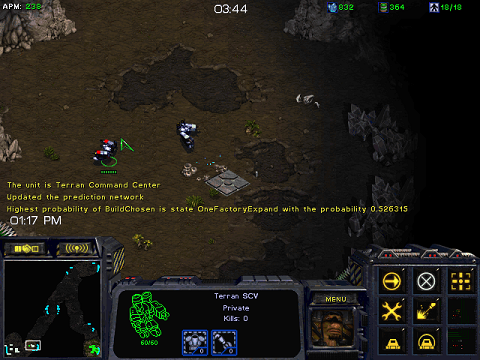
\includegraphics[scale=0.7]{Figures/BuildOrderPredictorTest/Predicting.png}
		\caption{Predicting one fact expand build upon seeing second command center}\label{fig:predicting}
		\end{center}
	\end{figure}
	\subsection{Prediction of Threatlevel test}
		In this test we wanted to see if the prediction network could analyze what he current threatlevel is based on what it sees and what the time is.
		The bot scouts the opponent and sees 2 hatcheries, which it predicts is going to be a 3 Hatch Muta build. Because that build is effective later 
		in the game the network predicts the current threatlevel to low. In the picture below (See \ref{fig:predicting}) this situation is shown. 
		This test just showed that the network worked exactly as assumed.
		\begin{figure}[H]
			\begin{center}
			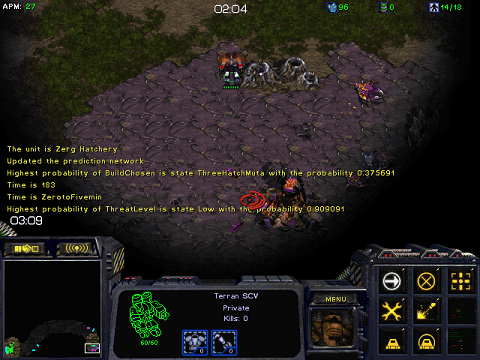
\includegraphics[scale=0.7]{Figures/BuildOrderPredictorTest/threatlevel.png}
			\caption{Predicting the current threatlevel}\label{fig:threatlevel}
			\end{center}
		\end{figure}